\documentclass{article}
\usepackage[utf8]{inputenc}
\usepackage{listings}
\usepackage{xcolor}
\usepackage{amsmath}
\usepackage{graphicx}
\usepackage{hyperref}
\definecolor{codegreen}{rgb}{0,0.6,0}
\definecolor{codegray}{rgb}{0.5,0.5,0.5}
\definecolor{codepurple}{rgb}{0.58,0,0.82}
\definecolor{backcolour}{rgb}{0.95,0.95,0.92}
\lstdefinestyle{mystyle}{
    commentstyle=\color{codegreen},
    keywordstyle=\color{magenta},
    numberstyle=\tiny\color{codegray},
    stringstyle=\color{codepurple},
    basicstyle=\ttfamily\footnotesize,
    breakatwhitespace=false,
    breaklines=true,
    captionpos=b,
    keepspaces=true,
    showspaces=false,
    showstringspaces=false,
    showtabs=false,
    tabsize=2
}
\lstset{style=mystyle}
\title{AGLA Assigment 3 Report}
\author{Anton Kudryavtsev CS-04}
\date{\today}
\begin{document}
\maketitle

\section*{Predator-Prey Model}
\graphicspath{ {./} }
\subsection*{k(t), v(t)}
\begin{lstlisting}
gnuplot> set xlabel "time"
gnuplot> set ylabel "population size"
gnuplot> plot
    "vt.dat" with points pt 7 ps 0.5 title "prey",
    "kt.dat" with points pt 7 ps 0.5 title "predator"
\end{lstlisting}
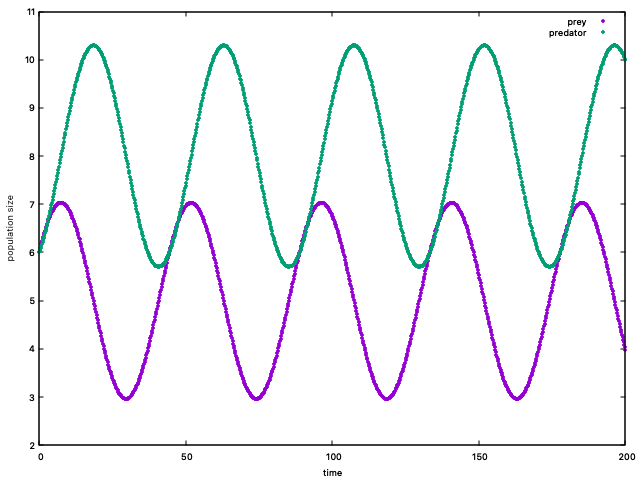
\includegraphics[scale=0.6]{vtkt.png}
\subsection*{k(v)}
\begin{lstlisting}
gnuplot> set xlabel "prey population size"
gnuplot> set ylabel "predator population size"
gnuplot> plot "kv.dat" with points pt 7 ps 0.5 title "predator"
\end{lstlisting}
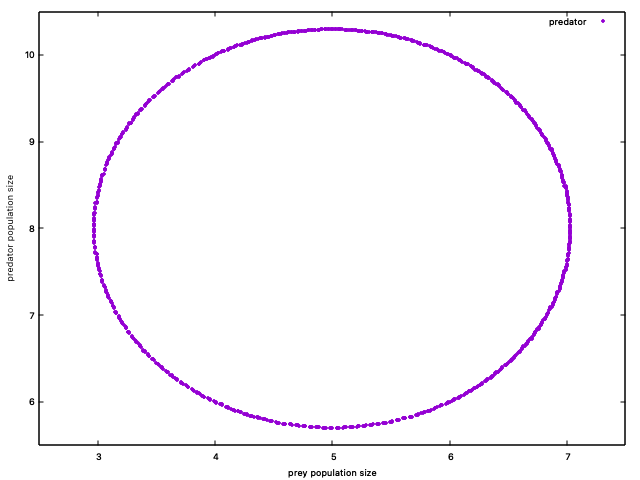
\includegraphics[scale=0.6]{kv.png}
\subsection*{v(k)}
\begin{lstlisting}
gnuplot> set xlabel "predator population size"
gnuplot> set ylabel "prey population size"
gnuplot> plot "vk.dat" with points pt 7 ps 0.5 title "prey"
\end{lstlisting}
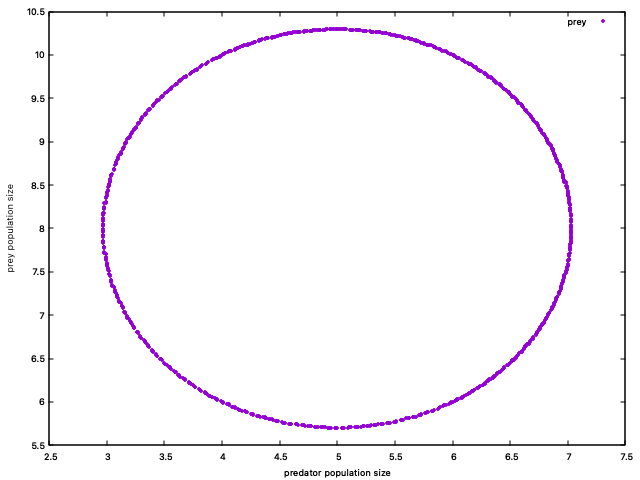
\includegraphics[scale=0.6]{vk.png}
\subsection*{Code}
\begin{lstlisting}[language=c++]
int main() {
    // Specify Output Format
    std::cout.setf(std::ios::fixed, std::ios::floatfield);
    std::cout.precision(2);

    // Input Parameters
    double alpha_1, alpha_2, beta_1, beta_2, v_0, k_0, t;
    int n;
    std::cin >> v_0 >> k_0 >> alpha_1 >> beta_1 >> alpha_2 >> beta_2 >> t >> n;


    double sample_time_span = t / n;
    double alpha_root = std::sqrt(alpha_1 * alpha_2);
    double predator_rate = (beta_1 * std::sqrt(alpha_2)) / (beta_2 * std::sqrt(alpha_1));
    double prey_rate = 1 / predator_rate;

    // U = [V, K, 1], U0 = [V0, K0, 1], V0 = v_0 - alpha_2/beta_2, K0 = k_0 - alpha_1/beta_1;
    // U(t) = eAt*U0

    // dU = A(2x2) *u(2x1) + b(2x1); => dU = A(3x3)*u(3x1);
    // dU = [ a1 a2 a3        [ v
    //        a4 a5 a6    *     k
    //         0  0  0 ]        1 ]

    Matrix<double> *U_0 = new ColumnVector<double>(3);

    U_0->Put(0, 0, v_0 - alpha_2 / beta_2);
    U_0->Put(1, 0, k_0 - alpha_1 / beta_1);
    U_0->Put(2, 0, 1);


    // Coefficients from analytical solution of ODE in general form
    auto eA = [alpha_root, predator_rate, prey_rate, alpha_2, beta_2, alpha_1, beta_1](double t) {
        auto m = new SquareMatrix<double>(3);

        // Prey gain from their population
        m->Put(0, 0, std::cos(alpha_root * t));
        // Prey lose from meetings with predators
        m->Put(0, 1, -predator_rate * std::sin(alpha_root * t));
        // Free coefficient in ODE
        m->Put(0, 2, alpha_2 / beta_2);

        // Predators gain from meetings with preys
        m->Put(1, 0, prey_rate * sin(alpha_root * t));
        // Predators lose from their population
        m->Put(1, 1, cos(alpha_root * t));
        // Free coefficient in ODE
        m->Put(1, 2, alpha_1 / beta_1);

        // Last row 0-s
        m->Put(2, 0, 0);
        m->Put(2, 1, 0);
        m->Put(2, 2, 0);

        return m;
    };

    auto time_series = std::vector<double>(n+1, 0);
    auto prey_population = std::vector<double>(n+1, 0);
    auto predator_population = std::vector<double>(n+1, 0);

    for (int i = 0; i < n + 1; i++) {
        auto ti = sample_time_span * i;

        auto eAt = eA(ti);
        auto Ui = *eAt * U_0;

        time_series[i] = ti;
        prey_population[i] = Ui->Get(0, 0);
        predator_population[i] = Ui->Get(0, 1);

        free({eAt, Ui});
    }

    std::cout << "t:" << std::endl;
    for (auto x: time_series) std::cout << x << " ";
    std::cout << std::endl;

    std::cout << "v:" << std::endl;
    for (auto x: prey_population) std::cout << x << " ";
    std::cout << std::endl;

    std::cout << "k:" << std::endl;
    for (auto x: predator_population) std::cout << x << " ";
    std::cout << std::endl;

    free({U_0});
    return 0;
}
\end{lstlisting}

Complete code available here: : \href{https://github.com/Dartt0n/Least-Square-Approximation-Cpp}{Github}
\end{document}